\section{Cross Validation} \label{sc:crossValidation}
Cross validation is a technique for model validation. A model is normally trained on parts of a dataset and later another part of the dataset of unknown data will be tested against the model. With cross validation the aim is to use the the training set in the model in the training to limit problems like overfitting and help gain insight on how the model will behave to a never seen before dataset. There is several options for Cross Validation. The following sections will describe Validation set approach, Leave one out cross validation and K-fold what is the techniques used here.

\section{Validation set approach}
\subsection{Theory}
The Validation set approach works by splitting the data to two parts one is called the training set and the other is called the testing set(validation or hold-out set). An example of the split can be seen on Figure \ref{fig:validationsetapproach}. The model is trained with the training set, after the training is finished the model is tested with the testing set, which the model was not trained on. This test produces a test error, in the form of MSE, which is good for validating the model. The advantage of this method is low computation time, but the results of this method is depended on which data points will end up in the sets. 
\begin{figure}[H]
	\centering
	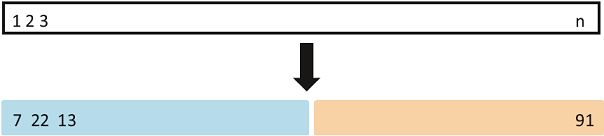
\includegraphics[width=0.4\linewidth]{crossValidation/validationSetApproach}
	\caption{Validation set approach. The entire dataset is split randomly into a training and testing set.}
	\label{fig:validationsetapproach}
\end{figure}

\subsection{Result}
\subsubsection*{LAB 5.3.1}%TODO write full lab
In lab 5.3.1 the validation set approach is used to find estimate the test error that result from fitting linear models on the Auto data\footnote{https://raw.github.com/vincentarelbundock/Rdatasets/master/csv/ISLR/Auto.csv} set.

Then we are fiting linear model on our training set and testing our model with the test data.


As we can see below the MSE is quit high.
\begin{lstlisting}
23.36190289258723
\end{lstlisting}
We can reduce the MSE with polynomial or cubic regression.

The out put:
\begin{lstlisting}[language=Python]
--------Test Error for 2nd order--------
20.25269085835005
--------Test Error for 3rd order--------
20.325609365773605
\end{lstlisting}
As we can see we are starting to reach the overfilling line with the cubic Polynomial. 

\section {Leave one out cross validation}

\subsection{Theory}
This type of cross validation is used when there is limited amount of data. It works the same way as k-fold cross validation, but instead subset we are using signal data entry, that means K is N in this case.The mathematic formula is below. 

\begin{figure}[H]
	\centering
	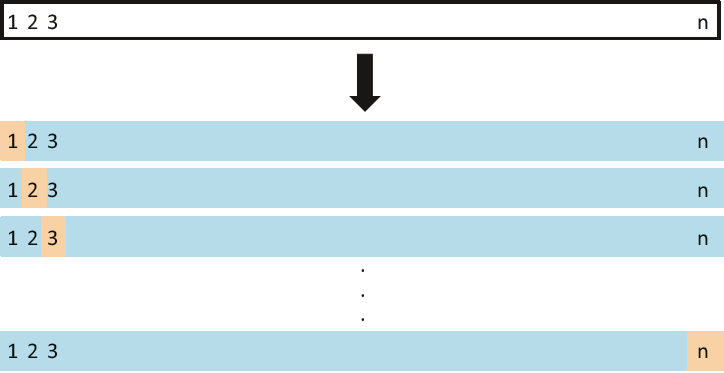
\includegraphics[width=0.5\linewidth]{crossValidation/LOOCV}
	\caption{}
	\label{fig:loocv}
\end{figure}


\begin{align}\label{fo:LOOCV}
CV_{(n)} = \frac {1}{n} \sum_{k=1}^{K}  (\frac {y_i-\hat{y_i}}{1- h_i})^2
\end{align}



\subsection{Result}
In lab 3.4.2 we had the same auto data. We used the LOOCV method to find MSE. We made an algorithm for this method, because we coul not find a library for this method.

\begin{lstlisting}[language=Python]
X = df["horsepower"].values.reshape(-1,1)
y = df["mpg"].values.reshape(-1,1) 

loo = LeaveOneOut()
print('Splits: ', loo.get_n_splits(X))

ytests = []
ypreds = []

for train_index, test_index in loo.split(X):
X_train, X_test = X[train_index], X[test_index]
y_train, y_test = y[train_index], y[test_index]

model = linear_model.LinearRegression()
model.fit(X = X_train, y = y_train)
y_pred = model.predict(X_test)

ytests += list(y_test)
ypreds += list(y_pred)

rr = metrics.r2_score(ytests, ypreds)
ms_error = metrics.mean_squared_error(ytests, ypreds)

print("LOOCV results:")
print("R^2: {:.5f}%, MSE: {:.5f}".format(rr*100, ms_error))
\end{lstlisting}

The output:
\begin{lstlisting}[language=Python]
Splits:  392
LOOCV results:
R^2: 60.12110%, MSE: 24.23151
\end{lstlisting}

As we can see our algorithm has worked.Also we have seen a mass increased computing time in the machine. It was expected, because of retraining and revalidating the model 392 time.

\section {K-fold cross validation}%TODO explain in more detail (give pictures)
\subsection{Theory}
In this type of cross validation the split the data k-subsets and we repeat validation set approach for k times. In each time we take one subest as a test set and other combine are training set. After all copulations we compute average error. The advantage of this method is that all data points are one time in the testing set. The drift of the test is reduced when k is increasing. We can choose the k value, most oftenly k values are 5 or 10 . The disadvantages is that we have to retrain the model k times and the computation time increases. The mathematic formula is below. 
\begin{align}\label{fo:k-fold}
CV_{(K)} = \sum_{k=1}^{K}  \frac {n_{k}}{n}MSE_{(k)}
\end{align}

\subsection{Result}
\subsubsection*{LAB 5.3.3}%TODO write full lab
In the lab 5.3.3 we used K-fold cross validation find the MSE. We are using auto data from the book. In this particular case we are using k = 10. 
\begin{lstlisting}[language=Python]
from sklearn.model_selection import KFold

X = Data["horsepower"].values.reshape(-1,1) 
y = Data["mpg"].values.reshape(-1,1)
kf= KFold()
kf.n_splits = 10
\end{lstlisting}
Now we need to make a loop for all the folds to calculate MSE.   

\begin{lstlisting}[language=Python]
ytests = []
ypreds = []

for train_index, test_index in kf.split(Data):
	X_train, X_test = X[train_index], X[test_index]
	y_train, y_test = y[train_index], y[test_index]

	model = linear_model.LinearRegression()
	model.fit(X = X_train, y = y_train)
	y_pred = model.predict(X_test)  
	ypreds += list(y_pred)
	ytests += list(y_test)
	ms_error = metrics.mean_squared_error(ytests, ypreds)
	print("%.2f" %ms_error, end=" ")
\end{lstlisting}
Out put of the code is:
\begin{lstlisting}[language=Python]
28.35 22.79 24.14 23.95 22.29 21.56 20.92 21.16 26.11 27.42 
\end{lstlisting}
Having all MSE we can choose the best model from the results. or 